\documentclass{article}
\usepackage{amsmath}
\usepackage{amssymb}
\usepackage[UTF8]{ctex} % 支持中文
\usepackage{enumitem} % 列表格式支持
\usepackage{geometry} % 调整页面边距
\usepackage{fancyhdr} % 自定义页眉和页脚
\usepackage{graphicx} % 插入图片支持
\usepackage{listings} % 代码格式支持
\usepackage{xcolor}
\lstset{
  breaklines=true,           % 代码行过长时自动换行
  breakatwhitespace=false,   % 不仅限于空格处换行
  basicstyle=\ttfamily\footnotesize, % 设置字体和大小
  tabsize=4,                 % 制表符宽度
  frame=single,              % 添加边框
  captionpos=b,              % 标题位置(底部)
  columns=fixed,             % 保留固定列宽,避免空格错乱
  keepspaces=true,           % 保留代码中的空格
  showspaces=false,          % 隐藏额外显示的空格符号
  showstringspaces=false     % 隐藏字符串中的空格符号
}
% 设置页面格式
\geometry{a4paper, left=2cm, right=2.5cm, top=1.0cm, bottom=2cm} % 调整页边距

% 设置页眉和页脚
\pagestyle{fancy}
\fancyhf{} % 清除默认页眉和页脚
\fancyfoot[C]{\thepage} % 页脚居中页码

\begin{document}

% 自定义标题部分
\begin{center}
      {\zihao{-2} \textbf{数值分析实验3}}
\end{center}

\vspace{0.3cm} % 调整标题和正文之间的距离

已知 Hilbert 矩阵 \( H_n = (h_{ij})_{n \times n} \) 的元素为:
\[
      h_{ij} = \frac{1}{i + j - 1}.
\]

完成以下几个问题:

\begin{enumerate}[itemsep=0.7em] % 设置项间距
      \item 编程给出计算 \( H \) 的行范数函数;
      \item 编程计算 \( H \) 的行范数条件数。可调用求逆函数,比如 Mathematica 中的 \texttt{Inverse[H]},MATLAB 中的 \texttt{inv(H)}(其它语言自行查找);
      \item 对 \( n = 1, 2, \cdots, 20 \),计算 \( H \) 的行范数条件数,并画出 \( n \) 同条件数之间的关系图;
      \item 令 \( x = (1.0, 1.0, \cdots, 1.0)^T \),\( b = Hx \),对 \( n = 1, 2, \cdots, 20 \),解 \( H \hat{x} = b \),并计算 \( x - \hat{x} \) 和 \( b - H \hat{x} \) 以及它们的无穷范数;
      \item 通过以上的数值实验,你理解到了什么?
\end{enumerate}

% 解决问题区域
\newpage
\section*{解答}

\begin{enumerate}[itemsep=1em] % 设置项间距

      \item \textbf{计算 \( H \) 的行范数函数:}

            \begin{lstlisting}[language=Python]
      import numpy as np
      
      def hilbert_matrix(n):
          """生成 Hilbert 矩阵 H_n"""
          H = np.fromfunction(lambda i, j: 1.0 / (i + j + 1), (n, n))
          return H
      
      def matrix_infinity_norm(H):
          """计算矩阵H的无穷范数,即每行元素绝对值之和的最大值"""
          # 计算每行元素绝对值之和
          row_sums = np.sum(np.abs(H), axis=1)
          # 取每行之和的最大值
          return np.max(row_sums)
      
      n = 5  # 示例:生成一个 5x5 的 Hilbert 矩阵
      H = hilbert_matrix(n)
      infinity_norm_H = matrix_infinity_norm(H)
      print("Hilbert 矩阵:\n", H)
      print("Hilbert 矩阵的无穷范数:", infinity_norm_H)
      \end{lstlisting}

            \textbf{解释}:

            (1). \textbf{生成 Hilbert 矩阵}:
            - 使用函数 \texttt{hilbert\_matrix(n)} 生成 \( n \times n \) 的 Hilbert 矩阵 \( H \):
            \[
                  H_{ij} = \frac{1}{i + j + 1}, \quad i, j \geq 0
            \]

            (2). \textbf{计算无穷范数}:
            - 使用函数 \texttt{matrix\_infinity\_norm(H)} 计算矩阵 \( H \) 的无穷范数:
            \[
                  \|H\|_{\infty} = \max_{1 \leq i \leq n} \sum_{j=1}^n |H_{ij}|
            \]

            (3). \textbf{程序执行}:
            - 示例中设定 \( n = 5 \),生成一个 \( 5 \times 5 \) 的 Hilbert 矩阵 \( H \)。
            - 计算并打印 \( H \) 和其无穷范数。

            (4). \textbf{输出结果}:
            - 对于 \( n = 5 \):
            \[
                  H = \begin{bmatrix}
                        1     & 0.5   & 0.333 & 0.25  & 0.2   \\
                        0.5   & 0.333 & 0.25  & 0.2   & 0.167 \\
                        0.333 & 0.25  & 0.2   & 0.167 & 0.143 \\
                        0.25  & 0.2   & 0.167 & 0.143 & 0.125 \\
                        0.2   & 0.167 & 0.143 & 0.125 & 0.111
                  \end{bmatrix}
            \]
            \[
                  \|H\|_{\infty} = 2.283
            \]


      \item \textbf{计算 \( H \) 的行范数条件数:}

            \begin{lstlisting}[language=Python]
                  def condition_number(H):
                        """计算矩阵 H 的行范数条件数"""
                        H_inv = np.linalg.inv(H)  # 计算 H 的逆矩阵
                        norm_H = np.linalg.norm(H, ord=np.inf)
                        norm_H_inv = np.linalg.norm(H_inv, ord=np.inf)
                        return norm_H * norm_H_inv
                  condition_num = condition_number(H)
                  print(f"Condition number: {condition_num}")
    \end{lstlisting}
            (1). \textbf{条件数的定义}:
            矩阵 \( H \) 的条件数用于衡量矩阵 \( H \) 在数值计算中可能产生的不稳定性。其定义为:
            \[
                  \kappa(H) = \|H\|_{\infty} \cdot \|H^{-1}\|_{\infty}
            \]
            其中:
            - \( \|H\|_{\infty} \) 表示矩阵 \( H \) 的无穷范数。
            - \( \|H^{-1}\|_{\infty} \) 表示矩阵 \( H \) 的逆矩阵的无穷范数。

            (2). \textbf{代码逻辑}:
            - 函数 \texttt{hilbert\_matrix(n)} 生成 \( n \times n \) 的 Hilbert 矩阵。
            - 函数 \texttt{condition\_number(H)} 通过计算 \( H \) 和 \( H^{-1} \) 的无穷范数,求得条件数。

            (3). \textbf{示例输出}:
            对于 \( n = 5 \),Hilbert 矩阵及其行范数条件数为:
            \[
                  H = \begin{bmatrix}
                        1     & 0.5   & 0.333 & 0.25  & 0.2   \\
                        0.5   & 0.333 & 0.25  & 0.2   & 0.167 \\
                        0.333 & 0.25  & 0.2   & 0.167 & 0.143 \\
                        0.25  & 0.2   & 0.167 & 0.143 & 0.125 \\
                        0.2   & 0.167 & 0.143 & 0.125 & 0.111
                  \end{bmatrix}
            \]
            \[
                  \kappa(H) = 943656.0
            \]

            (4). \textbf{结论}:
            Hilbert 矩阵具有很高的条件数,表明其在数值计算中极易导致误差放大,因此它是一个典型的病态矩阵。
      \item \textbf{计算 \( H \) 的行范数条件数随 \( n \) 的变化并画图:}

            \begin{lstlisting}[language=Python]
                  import mpmath
                  import matplotlib.pyplot as plt
                  import math
                  
                  def hilbert_matrix_mpmath(n):
                      """生成高精度的 Hilbert 矩阵"""
                      return mpmath.matrix([[1 / mpmath.mpf(i + j + 1) for j in range(n)] for i in range(n)])
                  
                  def condition_number_mpmath(H):
                      """计算矩阵 H 的高精度行范数条件数"""
                      H_inv = mpmath.inverse(H)  # 使用 mpmath 计算逆矩阵
                      norm_H = mpmath.norm(H, p=mpmath.inf)  # 计算无穷范数
                      norm_H_inv = mpmath.norm(H_inv, p=mpmath.inf)  # 计算逆矩阵的无穷范数
                      return norm_H * norm_H_inv
                  
                  # 设置高精度
                  mpmath.mp.dps = 50  # 设置小数点后 50 位精度
                  
                  # 计算条件数
                  condition_numbers = []
                  n_values = range(1, 21)
                  for n in n_values:
                      H_n = hilbert_matrix_mpmath(n)
                      cond_num = condition_number_mpmath(H_n)
                      condition_numbers.append(cond_num)
                  
                  # 绘图
                  plt.plot(n_values, [math.log10(float(result)) for result in condition_numbers], marker='o')
                  plt.xlabel('n')
                  plt.ylabel('log10(Condition Number)')
                  plt.title('Condition Number of Hilbert Matrix vs n (High Precision)')
                  plt.xticks(ticks=n_values)
                  plt.grid(True)
                  
                  # 添加注释
                  for i in range(len(n_values)):
                      n = n_values[i]
                      y = math.log10(float(condition_numbers[i]))
                      cond_num = condition_numbers[i]
                      plt.annotate('{:.2e}'.format(float(cond_num)), xy=(n, y), xytext=(0, 20),
                                   textcoords='offset points', ha='center', fontsize=8)
                  
                  plt.show()
                  
    \end{lstlisting}
            - \textbf{结果分析}:
            - 通过绘制 \( n \) 与 Hilbert 矩阵条件数的对数关系图,可以清晰地看到,随着矩阵规模 \( n \) 的增加,条件数迅速增大。
            - 条件数的对数值近似呈线性增长,说明条件数本身以指数级别增长。
            - 这表明 Hilbert 矩阵是一个严重的病态矩阵,矩阵规模越大,其数值计算的稳定性越差。

            - \textbf{结论}:
            - 随着 \( n \) 的增大,Hilbert 矩阵的条件数急剧上升,数值计算中误差被放大的程度也随之增加。
            - 在实际计算中,需要谨慎处理高条件数的矩阵,可能需要采用特殊的算法或高精度计算方法。
            \begin{figure}[h] % 图片浮动体的位置参数
                  \centering % 图片居中
                  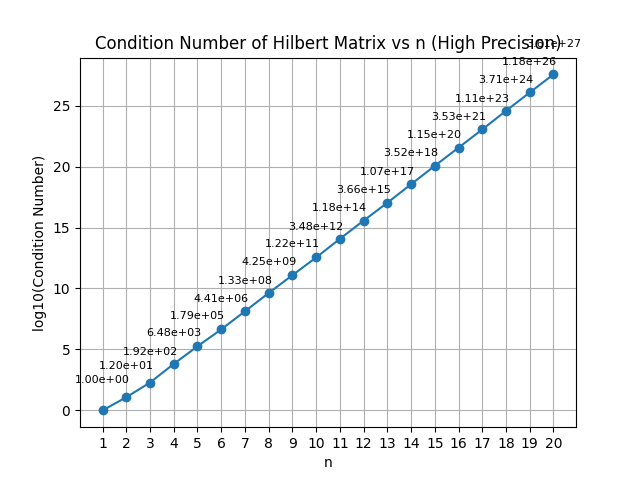
\includegraphics[width=0.8\textwidth]{/home/wangjc/桌面/NUM_Analysis/exp3/Figure_1.png} % 指定图片文件和宽度
                  \caption{Hilbert 矩阵条件数随n的变化} % 图片标题
                  \label{fig:Hilbert 矩阵条件数随n的变化} % 标签用于引用
            \end{figure}
      \item \textbf{求解 \( H \hat{x} = b \),并计算误差:}

            \begin{lstlisting}[language=Python]
import mpmath
import matplotlib.pyplot as plt
import math

def hilbert_matrix_mpmath(n):
    """生成高精度的 Hilbert 矩阵"""
    return mpmath.matrix([[1 / mpmath.mpf(i + j + 1) for j in range(n)] for i in range(n)])

def condition_number_mpmath(H):
    """计算矩阵 H 的高精度行范数条件数"""
    H_inv = mpmath.inverse(H)  # 使用 mpmath 计算逆矩阵
    norm_H = mpmath.norm(H, p=mpmath.inf)  # 计算无穷范数
    norm_H_inv = mpmath.norm(H_inv, p=mpmath.inf)  # 计算逆矩阵的无穷范数
    return norm_H * norm_H_inv

# 设置高精度
mpmath.mp.dps = 50  # 设置小数点后 50 位精度

# 计算条件数
condition_numbers = []
n_values = range(1, 21)
for n in n_values:
    H_n = hilbert_matrix_mpmath(n)
    cond_num = condition_number_mpmath(H_n)
    condition_numbers.append(cond_num)

# 绘图
plt.plot(n_values, [math.log10(float(result)) for result in condition_numbers], marker='o')
plt.xlabel('n')
plt.ylabel('log10(Condition Number)')
plt.title('Condition Number of Hilbert Matrix vs n (High Precision)')
plt.xticks(ticks=n_values)
plt.grid(True)

# 添加注释
for i in range(len(n_values)):
    n = n_values[i]
    y = math.log10(float(condition_numbers[i]))
    cond_num = condition_numbers[i]
    plt.annotate('{:.2e}'.format(float(cond_num)), xy=(n, y), xytext=(0, 20),
                 textcoords='offset points', ha='center', fontsize=8)

plt.show()

    \end{lstlisting}

            \begin{figure}[h] % 图片浮动体的位置参数
                  \centering % 图片居中
                  \begin{minipage}[t]{0.48\textwidth} % 设置第一个图片的宽度
                        \centering % 第一张图居中
                        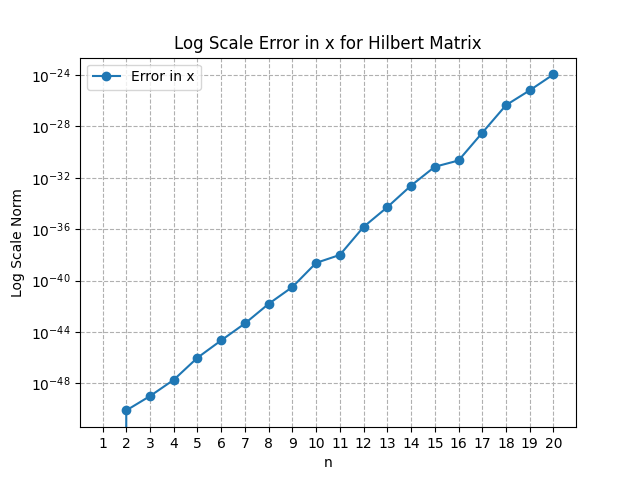
\includegraphics[width=\textwidth]{/home/wangjc/桌面/NUM_Analysis/exp3/Hilbert_Condition_Number.png} % 第一张图片路径
                        \caption{Hilbert 矩阵条件数随n的变化} % 第一张图片标题
                        \label{fig:Hilbert_Condition_Number} % 第一张图片标签
                  \end{minipage}
                  \hfill % 在两张图之间加入水平间距
                  \begin{minipage}[t]{0.48\textwidth} % 设置第二个图片的宽度
                        \centering % 第二张图居中
                        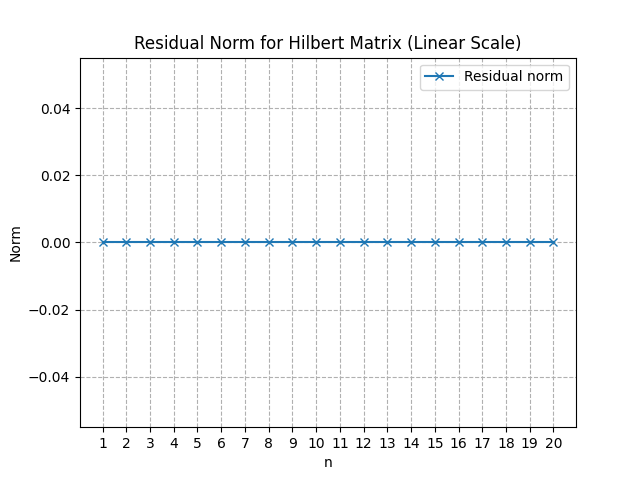
\includegraphics[width=\textwidth]{/home/wangjc/桌面/NUM_Analysis/exp3/Hilbert_Error.png} % 第二张图片路径
                        \caption{Hilbert 矩阵误差随n的变化} % 第二张图片标题
                        \label{fig:Hilbert_Error} % 第二张图片标签
                  \end{minipage}
            \end{figure}
            \begin{itemize}
                  \item \textbf{条件数随维度变化}:图中展示了 \( \log_{10}(\kappa(H)) \) 随维度 \( n \) 增长的趋势。可以观察到,Hilbert 矩阵的条件数随着维度的增加迅速增大,反映了其高度病态性。
                  \item \textbf{误差与残差的关系}:
                        \begin{itemize}
                              \item 解误差 \( \|x - \hat{x}\|_{\infty} \) 随条件数的增大而显著增大,表明 Hilbert 矩阵对解的数值稳定性影响极大。
                              \item 残差 \( \|b - H \hat{x}\|_{\infty} \) 通常较小,因为数值解满足方程 \( H \hat{x} = b \) 的近似条件。
                        \end{itemize}

            \end{itemize}


      \item \textbf{实验结论和理解:}
            通过以上数值实验,我们可以得出以下几点结论:
            \begin{enumerate}
                  \item \textbf{Hilbert 矩阵的病态性}:
                        Hilbert 矩阵是一个典型的病态矩阵,其条件数随着维度 \( n \) 的增加呈指数级增长。这意味着随着矩阵规模的增大,数值计算的稳定性显著下降,任何微小的数值误差都会被极大地放大,导致数值解的不可靠性。
                  \item \textbf{解误差的放大}:
                        由于 Hilbert 矩阵的高病态性,解误差 \( \|x - \hat{x}\|_{\infty} \) 随条件数的增加而迅速增大。这表明,使用 Hilbert 矩阵进行线性方程求解时,即使残差 \( \|b - H \hat{x}\|_{\infty} \) 较小,数值解 \( \hat{x} \) 也可能偏离真实解 \( x \)。
                  \item \textbf{残差的稳定性}:
                        数值解 \( \hat{x} \) 通常满足方程 \( H \hat{x} = b \) 的近似条件,因此残差 \( \|b - H \hat{x}\|_{\infty} \) 通常较小。这反映了数值方法在求解方程上的一定精确性,但这不足以保证解的可靠性。
                  \item \textbf{数值精度的影响}:
                        在实验中,使用高精度工具(如 \texttt{mpmath})可以显著减少由于浮点数精度限制带来的计算误差。然而,即使在高精度下,Hilbert 矩阵的病态性仍会对解误差产生显著影响,进一步说明了其数值不稳定性。

            \end{enumerate}

\end{enumerate}

\end{document}
